% Supplementary Note 1: sensitivity of survival dynamics to alpha and g.
%
% Standalone-compilable (paste the content between \begin{document} and
% \end{document} directly into the main manuscript's supplementary section
% if you'd rather not keep it as a separate file). Figure and table are
% generated by notebooks/99_parameter_sensitivity.py -- re-run that
% notebook and this file's \includegraphics/\input targets refresh in
% place, no manual editing of numbers required.
%
% Referenced from the main text as: "A sensitivity analysis of alpha and g
% around the DMSO baseline is given in Supplementary Note 1."

\documentclass[11pt]{article}
\usepackage[margin=1in]{geometry}
\usepackage{amsmath}
\usepackage{graphicx}
\usepackage{booktabs}
\usepackage{hyperref}

\newcommand{\supptitle}{Supplementary Note 1: Sensitivity of survival dynamics to the instability rate $\alpha$ and feedback strength $g$}

\begin{document}

\begin{center}
{\large \bfseries \supptitle}
\end{center}

\section*{Motivation}

A reviewer asked: \emph{``\ldots a parameter sensitivity analysis would be
useful. For example, what happens if only one parameter ($\alpha$ or $g$)
is changed at a time?''} The two coefficients enter the Langevin drift
asymmetrically, so there is no a priori reason to expect the survival
curve to respond to them in the same way. We quantify this directly by
perturbing $\alpha$ and $g$ one at a time around the fitted DMSO baseline
and comparing the resulting shift in simulated survival.

\section*{Model and baseline}

Organismal deterioration is modeled as the stochastic process (main text,
Eq.~1)
\begin{equation}
\frac{dz}{dt} = \alpha z + g z^2 + \sqrt{2D}\,\eta(t),
\label{eq:s1_langevin}
\end{equation}
integrated by Euler--Maruyama with fixed step $\Delta t = 0.1$ (matching
the step used to fit the main-text parameters),
$z(0) = 0$, and death defined as the first-passage event $z(t) \geq
Z \equiv \alpha/g$. The DMSO baseline used throughout the main text
(Table~I) is
\begin{equation}
\alpha_0 = 0.155\ \mathrm{d^{-1}}, \quad
g_0 = 2.86\times10^{-3}, \quad
Z_0 = \alpha_0/g_0 = 54.3, \quad
D = 1.27,
\label{eq:s1_baseline}
\end{equation}
with $D$ fixed at this value throughout, exactly as in the intervention
fits: the reviewer's question concerns $\alpha$ and $g$ specifically, and
holding $D$ fixed isolates their effect from the (separately estimated)
noise power.

It is useful to track the dimensionless ratio
\begin{equation}
\gamma \equiv \frac{\alpha Z^2}{2D},
\label{eq:s1_gamma}
\end{equation}
which sets the model's dynamical regime: $\gamma \gg 1$ is the
weak-nonlinearity, ``Gompertzian'' regime in which the population's
average lifespan greatly exceeds the intrinsic instability timescale
$\alpha^{-1}$ \cite{podolskiy2016}. All parameter combinations used to fit
the main-text conditions satisfy $\gamma \geq 50$.

\section*{Sweep design}

We perturb the baseline by a common set of multiplicative factors,
$\{0.5,\,0.75,\,1,\,1.25,\,1.5\}$ (i.e.\ $\pm 50\%$, $\pm 25\%$, and the
baseline itself), in two one-at-a-time sweeps:

\begin{itemize}
\item \textbf{Sweep A}: vary $\alpha$, hold $g=g_0$ fixed. Because
$Z = \alpha/g$, the failure threshold moves \emph{with} $\alpha$ in this
sweep.
\item \textbf{Sweep B}: vary $g$, hold $\alpha=\alpha_0$ fixed. $Z$ then
moves \emph{inversely} with $g$.
\end{itemize}

Substituting $Z=\alpha/g$ into Eq.~\eqref{eq:s1_gamma} gives
$\gamma = \alpha^3/(2Dg^2)$, so \textbf{holding $g$ fixed, $\gamma$ scales
as $\alpha^3$}, while \textbf{holding $\alpha$ fixed, $\gamma$ scales as
$1/g^2$}. A cubic dependence is markedly steeper than an inverse-square
one over the same $\pm 50\%$ range, so Sweep A is expected to move the
survival curve considerably more than Sweep B -- a quantitative
prediction we check directly below rather than merely inspecting the
curves visually.

As an outcome metric we report the median simulated lifespan $T_{50}$
(the time at which the population's own simulated Kaplan--Meier curve
crosses $S=0.5$), rather than the mortality-rate doubling time
$\mathrm{MRDT}=\ln2/\alpha$: MRDT depends on $\alpha$ alone and is, by
construction, exactly unchanged across the entirety of Sweep B, even
though the survival curve itself visibly shifts (Fig.~\ref{fig:s1}, right
panel) -- reporting MRDT alone would make Sweep B look inert. $T_{50}$ is
obtained from direct stochastic simulation of
Eq.~\eqref{eq:s1_langevin} ($2\times10^4$ paths per parameter set), not
from the closed-form Gompertz survival function, because that closed form
is only derived to hold for $\gamma \gg 1$: Sweep A's $\alpha\times0.5$
point falls to $\gamma \approx 22.6$, below the $\gamma\geq50$ bound used
to constrain the main-text fits, where the closed-form approximation is
no longer guaranteed reliable.

\section*{Results}

\begin{figure}[htbp]
\centering
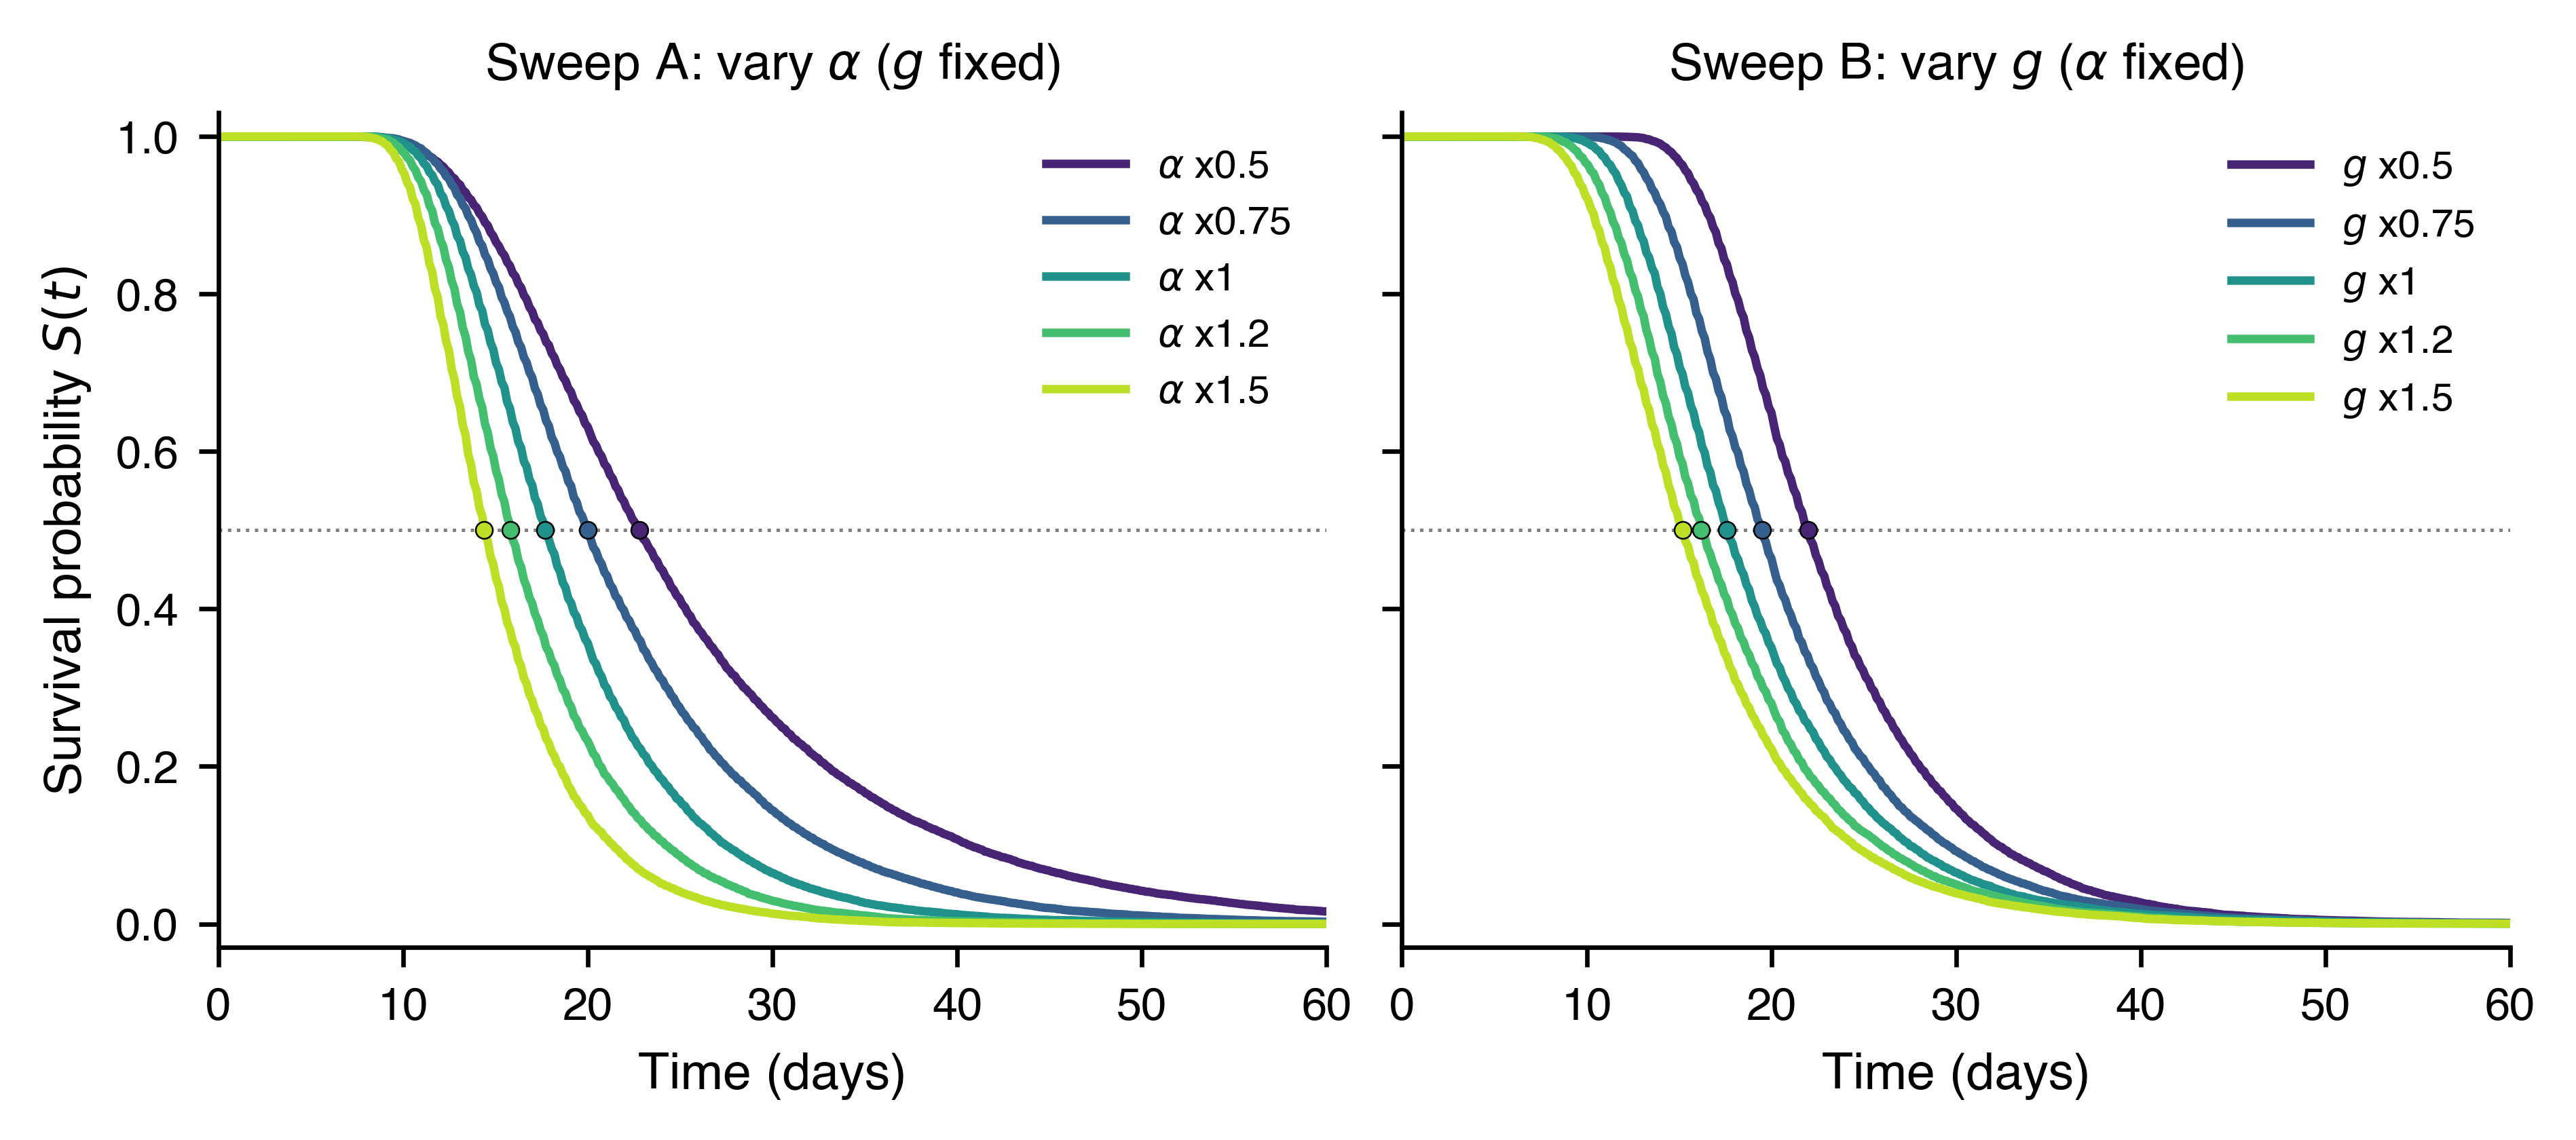
\includegraphics[width=\textwidth]{supp_note1_fig.png}
\caption{Simulated Kaplan--Meier survival curves under one-at-a-time
perturbation of $\alpha$ (left) or $g$ (right), $\pm50\%$ and $\pm25\%$
around the DMSO baseline (teal). Circles mark each curve's median
survival time $T_{50}$. The $\alpha$ sweep visibly spreads the curves
more than the equivalent $g$ sweep.}
\label{fig:s1}
\end{figure}

% Auto-generated by notebooks/99_parameter_sensitivity.py -- do not edit by hand.
\begin{table}[htbp]
\centering
\begin{tabular}{lrrrrrr}
\toprule
Perturbation & Factor & $\alpha$ (d$^{-1}$) & $g$ ($10^{-3}$) & $Z_{max}$ & $T_{50}$ (d) & IQR (d) \\
\midrule
$\alpha$ varies & 0.5 & 0.0777 & 2.86 & 27.2 & 22.9 & 13.1 \\
$\alpha$ varies & 0.75 & 0.116 & 2.86 & 40.8 & 19.9 & 9.7 \\
$\alpha$ varies & 1 & 0.155 & 2.86 & 54.3 & 17.6 & 7.7 \\
$\alpha$ varies & 1.25 & 0.194 & 2.86 & 67.9 & 15.8 & 6.2 \\
$\alpha$ varies & 1.5 & 0.233 & 2.86 & 81.5 & 14.4 & 5.2 \\
\midrule
$g$ varies & 0.5 & 0.155 & 1.43 & 108.7 & 22.0 & 7.9 \\
$g$ varies & 0.75 & 0.155 & 2.14 & 72.4 & 19.4 & 7.7 \\
$g$ varies & 1 & 0.155 & 2.86 & 54.3 & 17.6 & 7.7 \\
$g$ varies & 1.25 & 0.155 & 3.57 & 43.5 & 16.3 & 7.4 \\
$g$ varies & 1.5 & 0.155 & 4.29 & 36.2 & 15.2 & 7.3 \\
\bottomrule
\end{tabular}
\caption{One-at-a-time sensitivity of survival to $\alpha$ and $g$. Each parameter scaled by the given factor around the DMSO baseline ($\alpha_0=0.155$~d$^{-1}$, $g_0=2.86\times10^{-3}$, $Z_{max,0}=54.3$) with the other held fixed. $D=1.27$ throughout. $T_{50}$ is the median of $2\times10^4$ simulated first-passage times (Euler--Maruyama, $\Delta t=0.1$); IQR is $T_{25}-T_{75}$, the interquartile range of the same simulated lifespans.}
\label{tab:supp_note1_sensitivity}
\end{table}


Table~\ref{tab:supp_note1_sensitivity} confirms the prediction
numerically: across the full $\pm50\%$ range, Sweep A spans $T_{50} \in
[14.4,\,22.9]$~d (range $8.5$~d) while Sweep B spans $T_{50} \in
[15.2,\,22.0]$~d (range $6.8$~d). $\gamma$ likewise swings far more under
Sweep A ($22.6$ to $609$) than under Sweep B ($80.2$ to $722$), consistent
with the $\alpha^3$ vs.\ $1/g^2$ scaling derived above.

\section*{Conclusion}

$\alpha$ is the more powerful lever on survival outcome in this model:
equal relative perturbations to $\alpha$ shift the median lifespan more
than equivalent perturbations to $g$, a direct, derivable consequence of
how the two coefficients enter the dimensionless regime parameter
$\gamma$ once $Z=\alpha/g$ is substituted in. This is not a symmetry one
should expect a priori from the drift equation's literal coefficients,
and it is consistent with the fitting procedure's own emphasis on
$\alpha$ as the primary determinant of each condition's survival curve
(main text, Table~I).

\begin{thebibliography}{9}
\bibitem{podolskiy2016}
D.~Podolskiy, I.~Molodtcov, A.~Zenin, V.~Kogan, L.~I.~Menshikov,
V.~N.~Gladyshev, \emph{et al.}, \emph{Critical dynamics of gene networks
is a mechanism behind aging and Gompertz law}, arXiv:1502.04307 (2016).
\end{thebibliography}

\end{document}
